\documentclass[twoside]{book}

% Packages required by doxygen
\usepackage{fixltx2e}
\usepackage{calc}
\usepackage{doxygen}
\usepackage[export]{adjustbox} % also loads graphicx
\usepackage{graphicx}
\usepackage[utf8]{inputenc}
\usepackage{makeidx}
\usepackage{multicol}
\usepackage{multirow}
\PassOptionsToPackage{warn}{textcomp}
\usepackage{textcomp}
\usepackage[nointegrals]{wasysym}
\usepackage[table]{xcolor}

% Font selection
\usepackage[T1]{fontenc}
\usepackage[scaled=.90]{helvet}
\usepackage{courier}
\usepackage{amssymb}
\usepackage{sectsty}
\renewcommand{\familydefault}{\sfdefault}
\allsectionsfont{%
  \fontseries{bc}\selectfont%
  \color{darkgray}%
}
\renewcommand{\DoxyLabelFont}{%
  \fontseries{bc}\selectfont%
  \color{darkgray}%
}
\newcommand{\+}{\discretionary{\mbox{\scriptsize$\hookleftarrow$}}{}{}}

% Page & text layout
\usepackage{geometry}
\geometry{%
  a4paper,%
  top=2.5cm,%
  bottom=2.5cm,%
  left=2.5cm,%
  right=2.5cm%
}
\tolerance=750
\hfuzz=15pt
\hbadness=750
\setlength{\emergencystretch}{15pt}
\setlength{\parindent}{0cm}
\setlength{\parskip}{3ex plus 2ex minus 2ex}
\makeatletter
\renewcommand{\paragraph}{%
  \@startsection{paragraph}{4}{0ex}{-1.0ex}{1.0ex}{%
    \normalfont\normalsize\bfseries\SS@parafont%
  }%
}
\renewcommand{\subparagraph}{%
  \@startsection{subparagraph}{5}{0ex}{-1.0ex}{1.0ex}{%
    \normalfont\normalsize\bfseries\SS@subparafont%
  }%
}
\makeatother

% Headers & footers
\usepackage{fancyhdr}
\pagestyle{fancyplain}
\fancyhead[LE]{\fancyplain{}{\bfseries\thepage}}
\fancyhead[CE]{\fancyplain{}{}}
\fancyhead[RE]{\fancyplain{}{\bfseries\leftmark}}
\fancyhead[LO]{\fancyplain{}{\bfseries\rightmark}}
\fancyhead[CO]{\fancyplain{}{}}
\fancyhead[RO]{\fancyplain{}{\bfseries\thepage}}
\fancyfoot[LE]{\fancyplain{}{}}
\fancyfoot[CE]{\fancyplain{}{}}
\fancyfoot[RE]{\fancyplain{}{\bfseries\scriptsize Generated by Doxygen }}
\fancyfoot[LO]{\fancyplain{}{\bfseries\scriptsize Generated by Doxygen }}
\fancyfoot[CO]{\fancyplain{}{}}
\fancyfoot[RO]{\fancyplain{}{}}
\renewcommand{\footrulewidth}{0.4pt}
\renewcommand{\chaptermark}[1]{%
  \markboth{#1}{}%
}
\renewcommand{\sectionmark}[1]{%
  \markright{\thesection\ #1}%
}

% Indices & bibliography
\usepackage{natbib}
\usepackage[titles]{tocloft}
\setcounter{tocdepth}{3}
\setcounter{secnumdepth}{5}
\makeindex

% Custom commands
\newcommand{\clearemptydoublepage}{%
  \newpage{\pagestyle{empty}\cleardoublepage}%
}

\usepackage{caption}
\captionsetup{labelsep=space,justification=centering,font={bf},singlelinecheck=off,skip=4pt,position=top}

%===== C O N T E N T S =====

\begin{document}

% Titlepage & ToC
\pagenumbering{alph}
\begin{titlepage}
\vspace*{7cm}
\begin{center}%
{\Large Q\+T\+Supervisory }\\
\vspace*{1cm}
{\large Generated by Doxygen 1.8.14}\\
\end{center}
\end{titlepage}
\clearemptydoublepage
\pagenumbering{roman}
\tableofcontents
\clearemptydoublepage
\pagenumbering{arabic}

%--- Begin generated contents ---
\chapter{Namespace Index}
\section{Namespace List}
Here is a list of all namespaces with brief descriptions\+:\begin{DoxyCompactList}
\item\contentsline{section}{\textbf{ Ui} }{\pageref{namespace_ui}}{}
\end{DoxyCompactList}

\chapter{Hierarchical Index}
\section{Class Hierarchy}
This inheritance list is sorted roughly, but not completely, alphabetically\+:\begin{DoxyCompactList}
\item \contentsline{section}{Figura\+Geometrica}{\pageref{class_figura_geometrica}}{}
\begin{DoxyCompactList}
\item \contentsline{section}{Circulo}{\pageref{class_circulo}}{}
\item \contentsline{section}{Reta}{\pageref{class_reta}}{}
\item \contentsline{section}{Retangulo}{\pageref{class_retangulo}}{}
\end{DoxyCompactList}
\item \contentsline{section}{Screen}{\pageref{class_screen}}{}
\end{DoxyCompactList}

\chapter{Class Index}
\section{Class List}
Here are the classes, structs, unions and interfaces with brief descriptions\+:\begin{DoxyCompactList}
\item\contentsline{section}{\textbf{ Circulo} }{\pageref{class_circulo}}{}
\item\contentsline{section}{\textbf{ Figura\+Geometrica} }{\pageref{class_figura_geometrica}}{}
\item\contentsline{section}{\textbf{ Reta} }{\pageref{class_reta}}{}
\item\contentsline{section}{\textbf{ Retangulo} }{\pageref{class_retangulo}}{}
\item\contentsline{section}{\textbf{ Screen} }{\pageref{class_screen}}{}
\end{DoxyCompactList}

\chapter{File Index}
\section{File List}
Here is a list of all files with brief descriptions\+:\begin{DoxyCompactList}
\item\contentsline{section}{\textbf{ circulo.\+cpp} }{\pageref{circulo_8cpp}}{}
\item\contentsline{section}{\textbf{ circulo.\+h} }{\pageref{circulo_8h}}{}
\item\contentsline{section}{\textbf{ figurageometrica.\+cpp} }{\pageref{figurageometrica_8cpp}}{}
\item\contentsline{section}{\textbf{ figurageometrica.\+h} }{\pageref{figurageometrica_8h}}{}
\item\contentsline{section}{\textbf{ main.\+cpp} }{\pageref{main_8cpp}}{}
\item\contentsline{section}{\textbf{ reta.\+cpp} }{\pageref{reta_8cpp}}{}
\item\contentsline{section}{\textbf{ reta.\+h} }{\pageref{reta_8h}}{}
\item\contentsline{section}{\textbf{ retangulo.\+cpp} }{\pageref{retangulo_8cpp}}{}
\item\contentsline{section}{\textbf{ retangulo.\+h} }{\pageref{retangulo_8h}}{}
\item\contentsline{section}{\textbf{ screen.\+cpp} }{\pageref{screen_8cpp}}{}
\item\contentsline{section}{\textbf{ screen.\+h} }{\pageref{screen_8h}}{}
\end{DoxyCompactList}

\chapter{Namespace Documentation}
\section{Ui Namespace Reference}
\label{namespace_ui}\index{Ui@{Ui}}

\chapter{Class Documentation}
\section{Main\+Window Class Reference}
\label{class_main_window}\index{Main\+Window@{Main\+Window}}


{\ttfamily \#include $<$mainwindow.\+h$>$}

Inheritance diagram for Main\+Window\+:\begin{figure}[H]
\begin{center}
\leavevmode
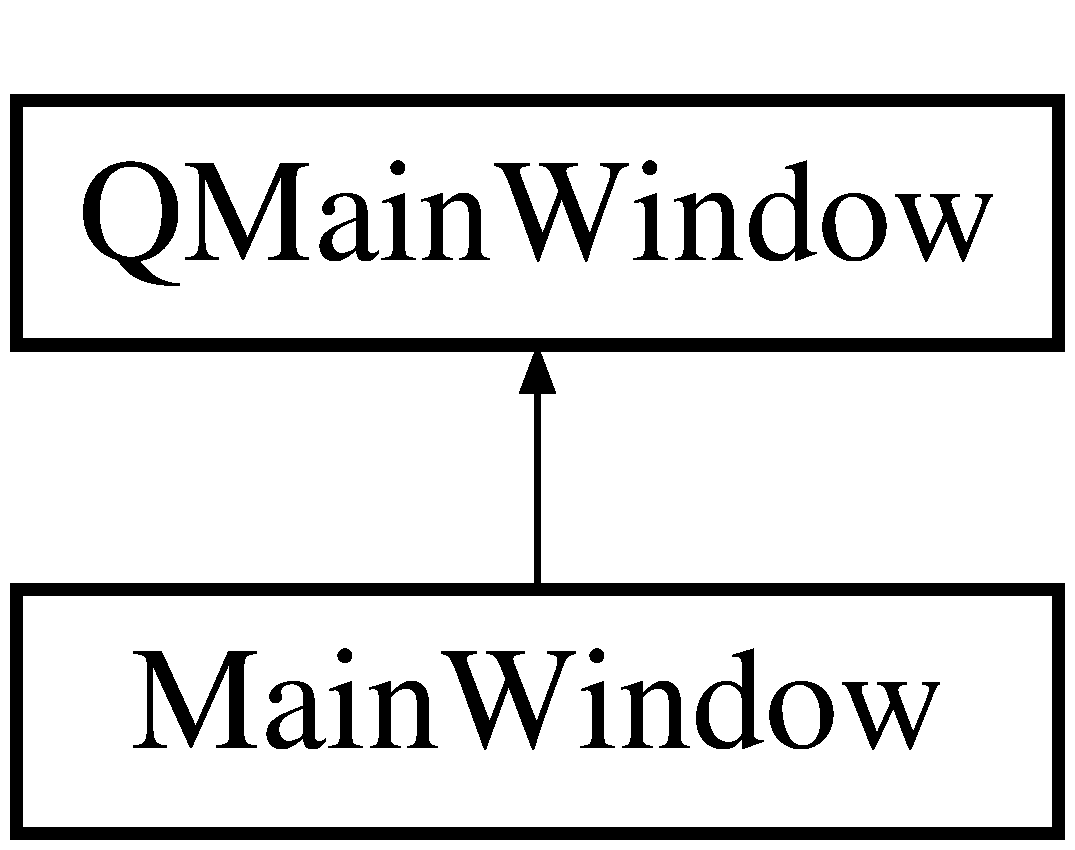
\includegraphics[height=2.000000cm]{class_main_window}
\end{center}
\end{figure}
\subsection*{Public Slots}
\begin{DoxyCompactItemize}
\item 
void \textbf{ tcp\+Connect} (void)
\begin{DoxyCompactList}\small\item\em \doxyref{Main\+Window\+::tcp\+Connect}{p.}{class_main_window_a26b6030035e196b64333906db8302cdd} -\/ Conecta com o servidor. \end{DoxyCompactList}\item 
void \textbf{ tcp\+Disconnect} (void)
\begin{DoxyCompactList}\small\item\em \doxyref{Main\+Window\+::tcp\+Disconnect}{p.}{class_main_window_a3389bbbe4222f115a7609037a1a63bd5} -\/ Disconecta do servidor. \end{DoxyCompactList}\item 
void \textbf{ get\+Data} (void)
\begin{DoxyCompactList}\small\item\em \doxyref{Main\+Window\+::get\+Data}{p.}{class_main_window_ac6d3a5fa8ef8ede69436b9e9a6ee80c1} -\/ Inicia a a captura de dados. \end{DoxyCompactList}\item 
void \textbf{ stop\+Data} (void)
\begin{DoxyCompactList}\small\item\em \doxyref{Main\+Window\+::stop\+Data}{p.}{class_main_window_a2e3dceeb08f18cc1d07e42b79fe7a0c1} -\/ Mata o temporizador e encerra o \doxyref{get\+Data()}{p.}{class_main_window_ac6d3a5fa8ef8ede69436b9e9a6ee80c1};. \end{DoxyCompactList}\item 
void \textbf{ update\+Ip} (void)
\begin{DoxyCompactList}\small\item\em Atualiza lista de clientes produtores conectados. \end{DoxyCompactList}\item 
void \textbf{ timer\+Event} (Q\+Timer\+Event $\ast$e)
\begin{DoxyCompactList}\small\item\em Time event. \end{DoxyCompactList}\end{DoxyCompactItemize}
\subsection*{Public Member Functions}
\begin{DoxyCompactItemize}
\item 
\textbf{ Main\+Window} (Q\+Widget $\ast$parent=0)
\item 
\textbf{ $\sim$\+Main\+Window} ()
\end{DoxyCompactItemize}


\subsection{Constructor \& Destructor Documentation}
\mbox{\label{class_main_window_a8b244be8b7b7db1b08de2a2acb9409db}} 
\index{Main\+Window@{Main\+Window}!Main\+Window@{Main\+Window}}
\index{Main\+Window@{Main\+Window}!Main\+Window@{Main\+Window}}
\subsubsection{Main\+Window()}
{\footnotesize\ttfamily Main\+Window\+::\+Main\+Window (\begin{DoxyParamCaption}\item[{Q\+Widget $\ast$}]{parent = {\ttfamily 0} }\end{DoxyParamCaption})\hspace{0.3cm}{\ttfamily [explicit]}}

\mbox{\label{class_main_window_ae98d00a93bc118200eeef9f9bba1dba7}} 
\index{Main\+Window@{Main\+Window}!````~Main\+Window@{$\sim$\+Main\+Window}}
\index{````~Main\+Window@{$\sim$\+Main\+Window}!Main\+Window@{Main\+Window}}
\subsubsection{$\sim$\+Main\+Window()}
{\footnotesize\ttfamily Main\+Window\+::$\sim$\+Main\+Window (\begin{DoxyParamCaption}{ }\end{DoxyParamCaption})}



\subsection{Member Function Documentation}
\mbox{\label{class_main_window_ac6d3a5fa8ef8ede69436b9e9a6ee80c1}} 
\index{Main\+Window@{Main\+Window}!get\+Data@{get\+Data}}
\index{get\+Data@{get\+Data}!Main\+Window@{Main\+Window}}
\subsubsection{get\+Data}
{\footnotesize\ttfamily void Main\+Window\+::get\+Data (\begin{DoxyParamCaption}\item[{void}]{ }\end{DoxyParamCaption})\hspace{0.3cm}{\ttfamily [slot]}}



\doxyref{Main\+Window\+::get\+Data}{p.}{class_main_window_ac6d3a5fa8ef8ede69436b9e9a6ee80c1} -\/ Inicia a a captura de dados. 

Pega os dados no intervalo de 30 em 30 amostras com um tempo determinado pelo usuário \mbox{\label{class_main_window_a2e3dceeb08f18cc1d07e42b79fe7a0c1}} 
\index{Main\+Window@{Main\+Window}!stop\+Data@{stop\+Data}}
\index{stop\+Data@{stop\+Data}!Main\+Window@{Main\+Window}}
\subsubsection{stop\+Data}
{\footnotesize\ttfamily void Main\+Window\+::stop\+Data (\begin{DoxyParamCaption}\item[{void}]{ }\end{DoxyParamCaption})\hspace{0.3cm}{\ttfamily [slot]}}



\doxyref{Main\+Window\+::stop\+Data}{p.}{class_main_window_a2e3dceeb08f18cc1d07e42b79fe7a0c1} -\/ Mata o temporizador e encerra o \doxyref{get\+Data()}{p.}{class_main_window_ac6d3a5fa8ef8ede69436b9e9a6ee80c1};. 

\mbox{\label{class_main_window_a26b6030035e196b64333906db8302cdd}} 
\index{Main\+Window@{Main\+Window}!tcp\+Connect@{tcp\+Connect}}
\index{tcp\+Connect@{tcp\+Connect}!Main\+Window@{Main\+Window}}
\subsubsection{tcp\+Connect}
{\footnotesize\ttfamily void Main\+Window\+::tcp\+Connect (\begin{DoxyParamCaption}\item[{void}]{ }\end{DoxyParamCaption})\hspace{0.3cm}{\ttfamily [slot]}}



\doxyref{Main\+Window\+::tcp\+Connect}{p.}{class_main_window_a26b6030035e196b64333906db8302cdd} -\/ Conecta com o servidor. 

\mbox{\label{class_main_window_a3389bbbe4222f115a7609037a1a63bd5}} 
\index{Main\+Window@{Main\+Window}!tcp\+Disconnect@{tcp\+Disconnect}}
\index{tcp\+Disconnect@{tcp\+Disconnect}!Main\+Window@{Main\+Window}}
\subsubsection{tcp\+Disconnect}
{\footnotesize\ttfamily void Main\+Window\+::tcp\+Disconnect (\begin{DoxyParamCaption}\item[{void}]{ }\end{DoxyParamCaption})\hspace{0.3cm}{\ttfamily [slot]}}



\doxyref{Main\+Window\+::tcp\+Disconnect}{p.}{class_main_window_a3389bbbe4222f115a7609037a1a63bd5} -\/ Disconecta do servidor. 

\mbox{\label{class_main_window_a9d08a694a5f9c532225754381b8011ea}} 
\index{Main\+Window@{Main\+Window}!timer\+Event@{timer\+Event}}
\index{timer\+Event@{timer\+Event}!Main\+Window@{Main\+Window}}
\subsubsection{timer\+Event}
{\footnotesize\ttfamily void Main\+Window\+::timer\+Event (\begin{DoxyParamCaption}\item[{Q\+Timer\+Event $\ast$}]{e }\end{DoxyParamCaption})\hspace{0.3cm}{\ttfamily [slot]}}



Time event. 

\doxyref{Main\+Window\+::timer\+Event}{p.}{class_main_window_a9d08a694a5f9c532225754381b8011ea} -\/ Configura o temporizador.

função que faz o \doxyref{get\+Data(void)}{p.}{class_main_window_ac6d3a5fa8ef8ede69436b9e9a6ee80c1} ser chamado no tempo determinado pelo usuário


\begin{DoxyItemize}
\item Configura o \doxyref{get\+Data()}{p.}{class_main_window_ac6d3a5fa8ef8ede69436b9e9a6ee80c1} de acordo com o intervalo fornecido pelo usuario 
\end{DoxyItemize}\mbox{\label{class_main_window_a6d5ab019a97676b4edfe7d4b6a541455}} 
\index{Main\+Window@{Main\+Window}!update\+Ip@{update\+Ip}}
\index{update\+Ip@{update\+Ip}!Main\+Window@{Main\+Window}}
\subsubsection{update\+Ip}
{\footnotesize\ttfamily void Main\+Window\+::update\+Ip (\begin{DoxyParamCaption}\item[{void}]{ }\end{DoxyParamCaption})\hspace{0.3cm}{\ttfamily [slot]}}



Atualiza lista de clientes produtores conectados. 

\doxyref{Main\+Window\+::update\+Ip}{p.}{class_main_window_a6d5ab019a97676b4edfe7d4b6a541455} -\/ Atualiza a lista de produtores conectados. 

The documentation for this class was generated from the following files\+:\begin{DoxyCompactItemize}
\item 
\textbf{ mainwindow.\+h}\item 
\textbf{ mainwindow.\+cpp}\end{DoxyCompactItemize}

\section{Plotter Class Reference}
\label{class_plotter}\index{Plotter@{Plotter}}


{\ttfamily \#include $<$plotter.\+h$>$}

Inheritance diagram for Plotter\+:\begin{figure}[H]
\begin{center}
\leavevmode
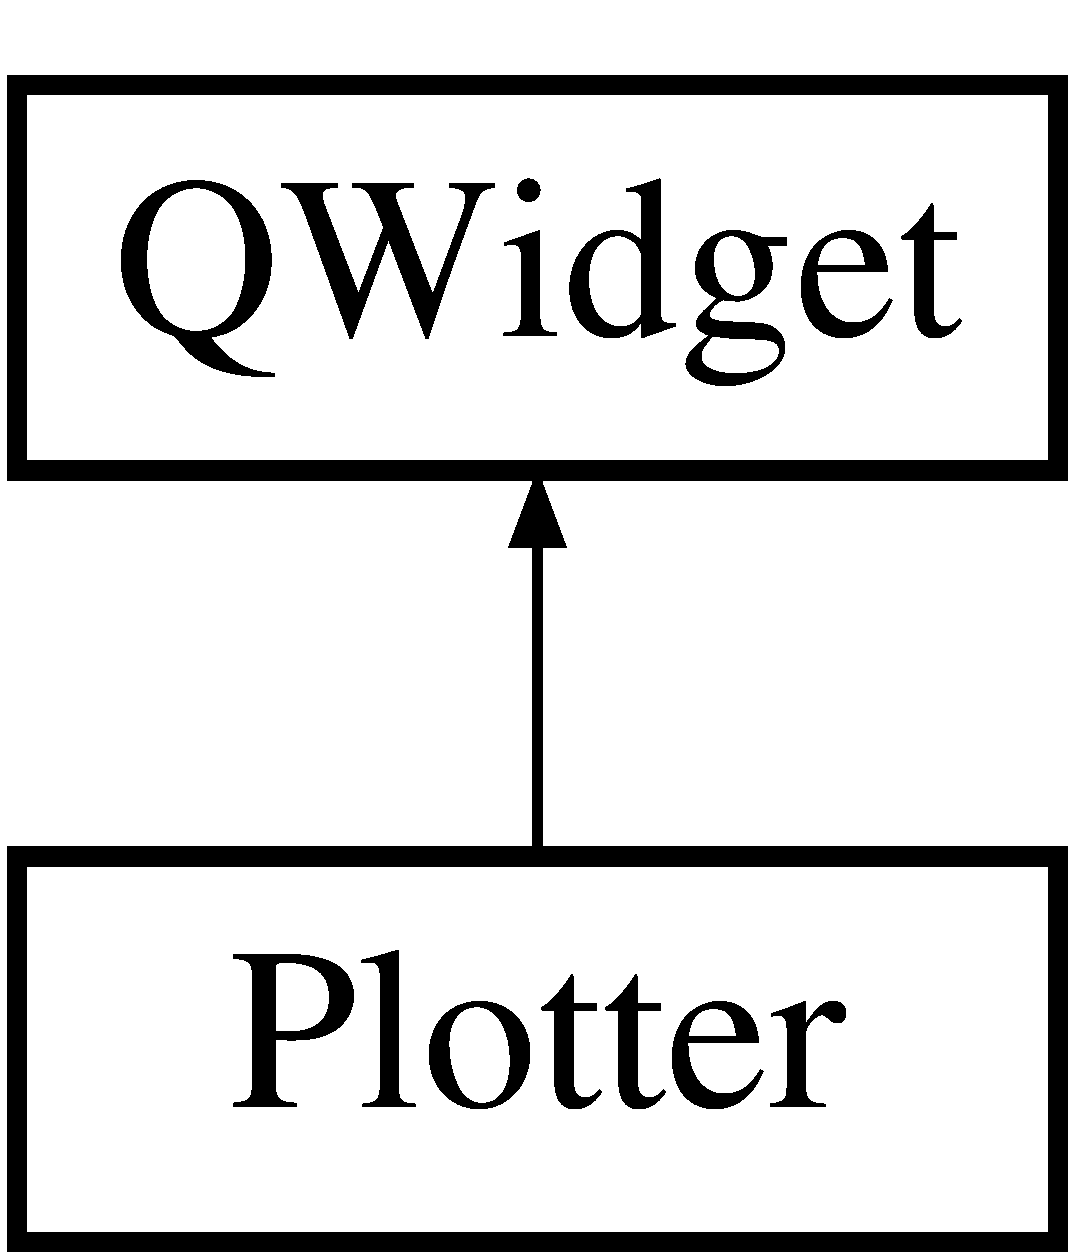
\includegraphics[height=2.000000cm]{class_plotter}
\end{center}
\end{figure}
\subsection*{Public Member Functions}
\begin{DoxyCompactItemize}
\item 
\textbf{ Plotter} (Q\+Widget $\ast$parent=0)
\begin{DoxyCompactList}\small\item\em Construtor do \doxyref{Plotter}{p.}{class_plotter}. \end{DoxyCompactList}\item 
void \textbf{ paint\+Event} (Q\+Paint\+Event $\ast$e)
\begin{DoxyCompactList}\small\item\em Paint event. \end{DoxyCompactList}\item 
void \textbf{ load\+Data} (std\+::vector$<$ double $>$, std\+::vector$<$ double $>$)
\begin{DoxyCompactList}\small\item\em Função que carrega dados. \end{DoxyCompactList}\end{DoxyCompactItemize}


\subsection{Constructor \& Destructor Documentation}
\mbox{\label{class_plotter_a367b6890c36910a27ec710ac3693e64b}} 
\index{Plotter@{Plotter}!Plotter@{Plotter}}
\index{Plotter@{Plotter}!Plotter@{Plotter}}
\subsubsection{Plotter()}
{\footnotesize\ttfamily Plotter\+::\+Plotter (\begin{DoxyParamCaption}\item[{Q\+Widget $\ast$}]{parent = {\ttfamily 0} }\end{DoxyParamCaption})\hspace{0.3cm}{\ttfamily [explicit]}}



Construtor do \doxyref{Plotter}{p.}{class_plotter}. 

\doxyref{Plotter\+::\+Plotter}{p.}{class_plotter_a367b6890c36910a27ec710ac3693e64b} -\/ Plota o grafico no intervalo de 30 em 30 dados.

seta valores aos vectors tempos e dados para evitar problemas com \char`\"{}lixos\char`\"{} 

\subsection{Member Function Documentation}
\mbox{\label{class_plotter_ae73b5093b98bbbebd6abdb4e7e7807ed}} 
\index{Plotter@{Plotter}!load\+Data@{load\+Data}}
\index{load\+Data@{load\+Data}!Plotter@{Plotter}}
\subsubsection{load\+Data()}
{\footnotesize\ttfamily void Plotter\+::load\+Data (\begin{DoxyParamCaption}\item[{std\+::vector$<$ double $>$}]{,  }\item[{std\+::vector$<$ double $>$}]{ }\end{DoxyParamCaption})}



Função que carrega dados. 

\doxyref{Plotter\+::load\+Data}{p.}{class_plotter_ae73b5093b98bbbebd6abdb4e7e7807ed} -\/ Captura os dados e envia para o plotter.

pega os 30 ultimos dados e envia para o paint\+Event


\begin{DoxyParams}{Parameters}
{\em t} & -\/ Vetor com os dados sobre o tempo \\
\hline
{\em d} & -\/ Vetor com dados capturados \\
\hline
\end{DoxyParams}
\mbox{\label{class_plotter_ac4341569909943e37e1ff756587e6e12}} 
\index{Plotter@{Plotter}!paint\+Event@{paint\+Event}}
\index{paint\+Event@{paint\+Event}!Plotter@{Plotter}}
\subsubsection{paint\+Event()}
{\footnotesize\ttfamily void Plotter\+::paint\+Event (\begin{DoxyParamCaption}\item[{Q\+Paint\+Event $\ast$}]{e }\end{DoxyParamCaption})}



Paint event. 

\doxyref{Plotter\+::paint\+Event}{p.}{class_plotter_ac4341569909943e37e1ff756587e6e12} -\/ Responsavel por desenhar o grafico.

desenha retas usando dois pontos por vez. Além disso, o eixo y para que a origem se encontre no canto inferior esquerdo. 

The documentation for this class was generated from the following files\+:\begin{DoxyCompactItemize}
\item 
\textbf{ plotter.\+h}\item 
\textbf{ plotter.\+cpp}\end{DoxyCompactItemize}

\chapter{File Documentation}
\section{main.\+cpp File Reference}
\label{main_8cpp}\index{main.\+cpp@{main.\+cpp}}
{\ttfamily \#include \char`\"{}mainwindow.\+h\char`\"{}}\newline
{\ttfamily \#include $<$Q\+Application$>$}\newline
\subsection*{Functions}
\begin{DoxyCompactItemize}
\item 
int \textbf{ main} (int argc, char $\ast$argv[$\,$])
\end{DoxyCompactItemize}


\subsection{Function Documentation}
\mbox{\label{main_8cpp_a0ddf1224851353fc92bfbff6f499fa97}} 
\index{main.\+cpp@{main.\+cpp}!main@{main}}
\index{main@{main}!main.\+cpp@{main.\+cpp}}
\subsubsection{main()}
{\footnotesize\ttfamily int main (\begin{DoxyParamCaption}\item[{int}]{argc,  }\item[{char $\ast$}]{argv[$\,$] }\end{DoxyParamCaption})}


\section{mainwindow.\+cpp File Reference}
\label{mainwindow_8cpp}\index{mainwindow.\+cpp@{mainwindow.\+cpp}}
{\ttfamily \#include \char`\"{}mainwindow.\+h\char`\"{}}\newline
{\ttfamily \#include \char`\"{}ui\+\_\+mainwindow.\+h\char`\"{}}\newline
{\ttfamily \#include $<$Q\+Date\+Time$>$}\newline
{\ttfamily \#include $<$Q\+Label$>$}\newline
{\ttfamily \#include $<$Q\+Line\+Edit$>$}\newline
{\ttfamily \#include $<$Q\+List\+Widget$>$}\newline
{\ttfamily \#include $<$Q\+Widget$>$}\newline
{\ttfamily \#include $<$Q\+Slider$>$}\newline
{\ttfamily \#include $<$vector$>$}\newline
{\ttfamily \#include $<$plotter.\+h$>$}\newline

\section{mainwindow.\+h File Reference}
\label{mainwindow_8h}\index{mainwindow.\+h@{mainwindow.\+h}}
{\ttfamily \#include $<$Q\+Main\+Window$>$}\newline
{\ttfamily \#include $<$Q\+Tcp\+Socket$>$}\newline
{\ttfamily \#include $<$Q\+Debug$>$}\newline
\subsection*{Classes}
\begin{DoxyCompactItemize}
\item 
class \textbf{ Main\+Window}
\end{DoxyCompactItemize}
\subsection*{Namespaces}
\begin{DoxyCompactItemize}
\item 
 \textbf{ Ui}
\end{DoxyCompactItemize}

\section{plotter.\+cpp File Reference}
\label{plotter_8cpp}\index{plotter.\+cpp@{plotter.\+cpp}}
{\ttfamily \#include \char`\"{}plotter.\+h\char`\"{}}\newline
{\ttfamily \#include $<$Q\+Painter$>$}\newline
{\ttfamily \#include $<$Q\+Brush$>$}\newline
{\ttfamily \#include $<$Q\+Pen$>$}\newline
{\ttfamily \#include $<$Q\+Color$>$}\newline
{\ttfamily \#include $<$cmath$>$}\newline
{\ttfamily \#include $<$Q\+Debug$>$}\newline

\section{plotter.\+h File Reference}
\label{plotter_8h}\index{plotter.\+h@{plotter.\+h}}
{\ttfamily \#include $<$Q\+Widget$>$}\newline
{\ttfamily \#include $<$vector$>$}\newline
\subsection*{Classes}
\begin{DoxyCompactItemize}
\item 
class \textbf{ Plotter}
\end{DoxyCompactItemize}

%--- End generated contents ---

% Index
\backmatter
\newpage
\phantomsection
\clearemptydoublepage
\addcontentsline{toc}{chapter}{Index}
\printindex

\end{document}
